\documentclass[9pt]{ctexbeamer}
\usepackage{tikz}
\usepackage{color}
\usepackage{graphicx}
\usepackage{ulem}

\linespread{1.2}
\newcommand{\setParDis}{\setlength{\parskip}{6pt}}
\newcommand{\rsa}{\rightsquigarrow}

\usetheme{Berlin}
\usefonttheme{professionalfonts,structurebold}

\title{2024 年第十届中国大学生程序设计竞赛(重庆)题解}
\author{清华大学}
\date{2024 年 11 月 10 日}

\begin{document}

\frame{\titlepage}

\section*{概况}

\begin{frame}
\setParDis
\begin{itemize}
	\item Easy: J, K, B, I, E
	\item Medium: C, D, A, M
	\item Hard: H, F, G, L
\end{itemize}
\end{frame}

\section{J}

\begin{frame}
\setParDis

J. 骰子

\begin{itemize}
	\item 考察如下三次骰子滚动的操作,其中绿色格子表示有骰子,格子上的数字是骰子顶面的数字而不是格子上写下的数字:
\end{itemize}
\centering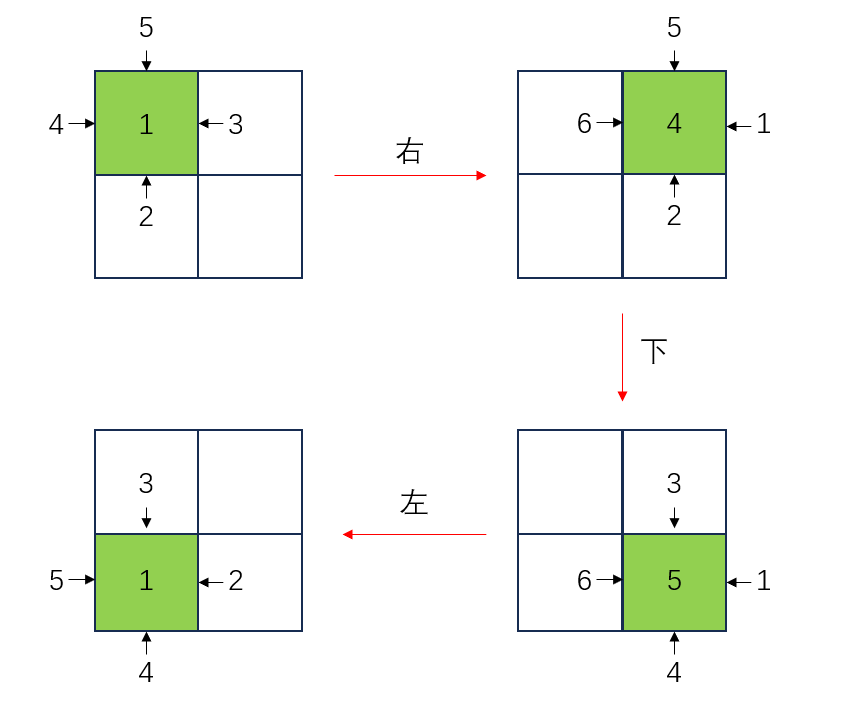
\includegraphics[width = 0.3 \textwidth]{J.png}
\begin{itemize}
	\item 由于我们只关心底面的数字,我们可以认为只要有 $2 \times 2$ 的空间,就可以让骰子在这个空间里进行任意的平移(实际上还会转一下但无所谓)。
	\item 因为 $n,m \ge 2$ 而且初始 6 在底面,所以可以直接让骰子平移到所有位置并在对应格子写下 6。显然没有更优方案,故输出 $6 \times n \times m$。
\end{itemize}

\end{frame}

\section{K}

\begin{frame}
\setParDis

K. 小 C 的神秘图形

\begin{itemize}
	\item 根据矩阵生成方式,可以发现:从高到低依次考虑每一个三进制位,如果 $n_1, n_2$ 在这一位上都不是 $1$ 则答案为 $0$,否则需要再判定下一位。
	\item 因此,当且仅当两个三进制数在每一位上都至少有一个是 $1$ 时答案为 $1$,否则为 $0$。
\end{itemize}

\end{frame}

\section{B}

\begin{frame}
\setParDis

B. osu!mania

\begin{itemize}
	\item 直接按照题目给出的公式模拟即可。
	\item 样例已经给出了可能出现精度误差的数据点,需要注意取整的方式:
	\begin{itemize}
		\item 一种方法是利用 $\operatorname{round}(x) = \lfloor x + 1 / 2 \rfloor$,然后转化为全整数计算;
		\item 另一种方法是直接在答案上加 $\text{eps}$,例如 $10 ^ {-6}$,然后直接四舍五入取整。
	\end{itemize}
\end{itemize}

\end{frame}

\section{I}

\begin{frame}
\setParDis

I. 算术

\begin{itemize}
	\item 首先,可以证明最终一定是分成若干组,每组分别求和,最终求积。
		\begin{itemize}
			\item 否则一定存在若干个积求和,这样是不优的。
			\item 例如 $a \times b + c$ 变成 $(a + c) \times b$ 一定不劣。
		\end{itemize}
	\item 之后可以证明每组里面不超过 $3$ 个数:
		\begin{itemize}
			\item 如果存在 $4$ 个,那分成两组并求积一定更优(每一组都 $\geq 2$)。
			\item 同理可得,每一组一定是 $x,x+1,1+1+1$ 中的一个。
			\item 所以每个 $1$ 要么 $1\sim 3$ 个组成一组,要么和一个其他的数分在一组。
		\end{itemize}
	\item 如果存在 $3$ 个组分别为 $x_1+1,x_2+1,x_3+1$($2 \le x_1, x_2, x_3 \le 9$):
		\begin{itemize}
			\item 考虑将其调整为 $x_1,x_2,x_3,1+1+1$ 三个组;
			\item 可以发现,除非 $x_1=x_2=x_3=2$,其他情况调整都是不劣的。
		\end{itemize}
		\item 如果存在 $3$ 个 $1+1$ 的组,调整为 $2$ 个 $1+1+1$ 的组更优($2 ^ 3 < 3 ^ 2$)。
\end{itemize}

\end{frame}

\begin{frame}
\setParDis

\begin{itemize}
	\item 一个避免分类讨论的写法:
		\begin{itemize}
			\item 如果同时存在 $1,2$ 则持续将 $1,2$ 变为 $3$。
			\item 如果此时存在三个 $1$ 则持续将 $1,1,1$ 变为 $3$。
			\item 如果此时仍有两个 $1$ 则将 $1,1$ 变为 $2$。
			\item 此时若仍存在 $1$,则找到其他数中最小的一个,将 $1$ 和这个数分到一组。
		\end{itemize}
\end{itemize}
\end{frame}

\section{E}

\begin{frame}
\setParDis

E. 合成大西瓜

\begin{itemize}
	\item 出题人的吐槽:选手们纷纷通过了此题,但是大家会证明自己的正确性吗?
	\item 结论是:
		\begin{itemize}
			\item 若权值最大的点度数不为一,那么答案就是权值的最大值;
			\item 否则是权值的非严格次大值。
		\end{itemize}
\end{itemize}

\end{frame}


\begin{frame}
\setParDis

\begin{itemize}
	\item 记权值最大,非严格次大值所在点为 $x,y$。
	\item 若 $x$ 的度数不为一:
		\begin{itemize}
			\item 取一棵以 $x$ 为根且 $x$ 度数大于一的生成树,在 $x$ 每棵子树内都尽可能地操作直到剩余不足三个点。接下来可以仅通过以 $x$ 为中心的操作消去其余所有点。
			\item 具体地,先不断消去大小为二的子树,这样可以把两棵大小为二的子树变成两个叶子,而且不影响 $x$ 的度数。接下来剩下至多一个大小为二的子树,任意操作后,再把剩余的叶子配对消去即可。
		\end{itemize}
	\item 若 $x$ 的度数为一且 $y$ 的度数不为一,效仿上述过程可以得到一个 $a_y$ 的解。
	\item 若 $x$ 与 $y$ 的度数均为一:
		\begin{itemize}
			\item 取 $x$ 到 $y$ 的一条路径,并在不影响路径上的点的情况下,尽可能消掉不在路径上的点。于是之后对于路径上每个点,其至多挂一个叶子。
			\item 接下来任取一个非链顶点的位置 $z$,满足 $z$ 的下方挂了一个叶子,那么此时 $z$ 的邻居必然有一个非 $x,y$ 的点(否则是四个点);
			\item 可以操作 $z$,叶子以及该邻居,并不断重复该操作直到仅剩一条两端点分别为 $x,y$ 的链,不断操作中心点即可让最后的点权为 $a_y$。
		\end{itemize}
\end{itemize}
\end{frame}

\section{C}

\begin{frame}
\setParDis

C. 连方

\begin{itemize}
	\item 若 $a,b$ 中恰有一个不含 \texttt{.},则无解。
	\item 若 $a,b$ 中均不含 \texttt{.},则将矩阵设为全 \texttt{\#}。
	\item 否则,按如下方式构造:
		\begin{itemize}
			\item $\{s_{2,i}\} = \{\texttt{\#}, \texttt{.}\} - \{a_i\}$(将第 $1$ 行中的 \texttt{\#} 通过第 $2$ 行连接);
			\item $\{s_{6,i}\} = \{\texttt{\#}, \texttt{.}\} - \{b_i\}$(将第 $7$ 行中的 \texttt{\#} 通过第 $6$ 行连接);
			\item 取任意 $l_1$ 满足 $s_{2, l_1} = \texttt{.} \land \left(s_{2, l_1 - 1} = \texttt{\#} \lor s_{2, l_1 + 1} = \texttt{\#}\right)$;
			\item 取任意 $l_2$ 满足 $s_{6, l_2} = \texttt{.} \land \left(s_{6, l_2 - 1} = \texttt{\#} \lor s_{6, l_2 + 1} = \texttt{\#}\right)$;
			\item 将 $s_{3, l_1}$ 和 $s_{5, l_2}$ 设为 $\texttt{\#}$,第三行与第五行其余位置设为 $\texttt{.}$;
			\item 将第 $3, 5$ 行的两个 $\texttt{\#}$ 通过第 $4$ 行连接即可。
		\end{itemize}
\end{itemize}

\end{frame}

\section{D}

\begin{frame}
\setParDis

D. 有限小数

\begin{itemize}
	\item 设 $L = 10 ^ 9$ 为 $d$ 的上界。
	\item 记 $w$ 为 $b$ 的最大的不能被 $2$ 或 $5$ 整除的因数。
	\item 下面证明最终答案的 $d$ 满足 $d=2^x5^yw$,其中 $x,y$ 是非负整数:
	\item 若存在质因数中不含 $2,5$ 的大于 $1$ 的正整数 $p$ 满足:
		\begin{itemize}
			\item[1.] $b$ 是 $p$ 的倍数而 $d$ 不是 $p$ 的倍数:
				\begin{itemize}
					\item 根据 $\gcd(a,b)=1$ 可得 $a$ 也不是 $p$ 的倍数,则 $p \mid bc,bd$ 而 $p \nmid ad$,
					\item 于是 $a / b + c / d = (ad+bc) / (bd)$ 不是有限小数。
				\end{itemize}
			\item[2.] $d$ 是 $p$ 的倍数而 $b$ 不是 $p$ 的倍数:
				\begin{itemize}
					\item 此时有 $p \mid ad, bd$,若 $(ad+bc) / (bd)$ 是整数或有限小数则 $p \mid bc$,
					\item 由 $p \nmid b$ 得 $p \mid c$,则 $\gcd(c, d) > 1$,不满足 $c$ 最小的条件。
				\end{itemize}
		\end{itemize}
	\item 综上,合法的 $d$ 的可能取值数不会超过 $O(\log ^ 2 L)$ 种。
	\item 枚举所有符合 $d=2^x5^yw$ 形式的 $d$,再分别解不定方程 $ad+bc=kbd$ 求出 $c$ 的最小非负整数解,最后取所有解中的最小值即可。
	\item 时间复杂度 $O(T\log^3 L)$。
\end{itemize}

\end{frame}

\section{A}

\begin{frame}
\setParDis

A. 乘积,欧拉函数,求和

\begin{itemize}
	\item 由 $\phi(x) = x \times \prod_{p \in \text{Prime}} [p \mid x] \frac{p-1}{p}$ 可得,所求即为 \[\sum_{S \subseteq [n]} \prod_{i \in S} a_i \prod_{p \in \text{Prime}} [p \mid \prod_{i \in S} a_i] \frac{p-1}{p}.\]
	\item 如果 $\prod_{i \in [n]} a_i$ 的质因子个数很少,不妨设其质因子集合为 $P$,可以对所有 $p \in P$ 记录 $[p \mid \prod_{i \in S} a_i]$ 是否为真,依次加入 $a_i$ 进行状压 DP:\[f_{j, Q} = \sum_{S \subseteq [j]} \prod_{i \in S} a_i [\forall p \in P, p \mid \prod_{i \in S} a_i \iff p \in Q],\]
	\item 即 $Q \subseteq P$ 记录了 $\prod_{i \in S} a_i$ 出现的质因子集合。
	\item 转移可以通过依次考虑是否加入 $a_1 \sim a_n$ 得到,答案即为 \[\sum_{Q \subseteq P} f_{n,Q} \prod_{p \in Q} \frac{p-1}{p}.\]
\end{itemize}

\end{frame}

\begin{frame}
\setParDis

\begin{itemize}
	\item 注意到如下事实:一个不超过 $V$ 的数至多有一个大于根号 $V$ 的因子。
	\item 因此大于根号 $V$ 的因子是否出现是“独立”的:要求某个 $p>\sqrt{V}$ 出现需要某个数集 $P \subseteq [n]$ 与选择的数集 $S$ 有交,而另一个 $q > \sqrt{V}$ 出现所限制的集合 $Q$ 一定是和 $P$ 无交的。
	\item 于是可以按照大于根号 $V$ 的因子归类输入的数,并一类一类地加入,进行以上 DP。对于每一类数对应的大于根号 $V$ 的因子 $p$,在转移时即可确定是否要计算 $p$ 的贡献 $\frac{p - 1}{p}$。
	\item 时间复杂度 $O(n 2 ^ {\omega(\sqrt{V})})$。
\end{itemize}

\end{frame}

\section{M}

\begin{frame}
\setParDis

M. Median Replacement

\begin{itemize}
	\item 首先考虑判断一个序列 $a$ 的值能否 $\ge x$:
		\begin{itemize}
			\item 将 $a$ 中 $\ge x$ 的数替换为 $1$,$<x$ 的数替换为 $0$,
			\item 则每次操作就是将选定区间中的所有数均替换为它们的众数。
			\item 可以发现当且仅当 $a$ 中存在两个 $1$ 的下标差 $\le 2$ 时,可将 $a$ 中所有数变为 $1$。
		\end{itemize}
	\item 接下来计算值 $\ge x$ 的序列个数,记之为 $c_x$:
		\begin{itemize}
			\item 考虑计算不存在两个 $1$ 的下标差 $\le 2$ 的序列个数 $c_x'$,则 \[c_x=\prod\limits_{i=1}^n(r_i-l_i+1)-c_x'.\]
			\item 使用动态规划求解 $c_x'$:
				\begin{itemize}
					\item 令 $f_{i,0/1/2}$ 表示仅考虑序列中前 $i$ 个数,且第 $i$ 位和第 $i-1$ 位分别 $(<x,<x)/(<x,\ge x)/(\ge x,<x)$ 的 $c_x'$ 的值。
					\item 转移可以通过将 $[l_i, r_i]$ 按 $x$ 分段得到。
				\end{itemize}
		\end{itemize}
\end{itemize}

\end{frame}

\begin{frame}
\setParDis

\begin{itemize}
	\item 回到原问题,值恰好等于 $x$ 的序列个数为 $c_x-c_{x+1}$,故所求即为 $\sum\limits_{x=1}^mc_x$。
	\item 考虑按所有的 $[l_i, r_i]$ 对值域进行分段。可以证明:对于每一段 $[l', r']$,均存在一个不超过 $n$ 次的多项式 $f(x)$,使得对于 $\forall x \in [l', r']$,$c_x = f(x)$。
	\item 进一步地,$\sum_{j = l'} ^ i c_j$ 是一个不超过 $n + 1$ 次的多项式 $g(x)$ 的点值 $g(i)$。
	\item 于是对于 $r' - l' + 1 \ge n + 2$ 的值域段,先计算出 $n + 2$ 个点值 \[c_{l'}, c_{l'} + c_{l' + 1}, \dots, c_{l'} + \dots + c_{l' + n + 1},\] 然后插值得到 $c_{l'} + \dots + c_{r'}$ 即可。
	\item 时间复杂度 $O(T n ^ 3)$。
\end{itemize}

\end{frame}

\section{H}

\begin{frame}
\setParDis

H. str(list(s))

\begin{itemize}
	\item 对于 $s ^ i$ 的第 $j$ 个字符:
		\begin{itemize}
			\item 当 $j \bmod p$ 确定时,$(5j + k) \bmod p$($0 \le k < p$)也是确定的,
			\item 于是可以直接将所有 $\bmod ~ p$ 相等的位置的信息记录下来。
		\end{itemize}
	\item 设计以下递推信息:
		\begin{itemize}
			\item $f_{i,j}$ 表示 $s^i$ 里下标 $\bmod ~ p=j$ 的位置的 ASCII 码和;
			\item 由于单引号转移与其他字符不同,因此还需要记录:
				\begin{itemize}
					\item $g_{i,j}$ 表示 $s^i$ 里下标 $\bmod ~ p=j$ 的位置中有多少个单引号,
					\item 以及 $h_{i,j}$ 表示 $s^i$ 里有多少个下标 $\bmod ~ p=j$ 的位置。
				\end{itemize}
		\end{itemize}
	\item $h$ 的转移是容易的。
\end{itemize}

\end{frame}

\begin{frame}
\setParDis

\begin{itemize}
	\item $f$ 可以直接按照题面描述进行转移(以下所有下标都在 $\bmod ~ p$ 意义下):
		\begin{itemize}
			\item $f_{i+1,5j+2} \to f_{i+1,5j+2}+f_{i,j}$,即复制自己;
			\item $f_{i+1,5j+3} \to f_{i+1,5j+3}+g_{i,j} \times 34 + (h_{i,j}-g_{i,j}) \times 39$,即单引号的位置加入双引号(ASCII 34),其他位置加入单引号(ASCII 39)。$f_{i+1,5j+1}$ 类似。
			\item $f_{i+1,5j} \to f_{i+1,5j} + h_{i,j} \times 32$,即所有位置都加入一个空格。$f_{i+1,5j+4}$ 类似。
			\item 特别地,需要处理左中括号与右中括号的贡献:
				\begin{itemize}
					\item 只需要在对应位置减掉一个空格再加上一个中括号;
					\item 左中括号的位置为 $0$,右中括号的位置需要用字符串长度 $\bmod ~ p$ 计算。
				\end{itemize}
		\end{itemize}
	\item $g$ 的转移也是类似的:
		\begin{itemize}
			\item $g_{i+1,5j+2} \leftarrow g_{i+1,5j+2} + g_{i,j}$,即复制自己;
				\begin{itemize}
					\item \sout{Fun Fact: 出题人和验题人最开始都漏掉了这个转移。}
					\item \textcolor{red}{这并不好笑。我们直到最后半个小时才发现大样例传的是错误的旧版本。对此我们感到非常抱歉,希望没有对比赛产生太多影响。}
				\end{itemize}
			\item $g_{i+1,5j+3} \leftarrow g_{i+1,5j+3} + (h_{i,j}-g_{i,j})$,即当自己不是单引号的时候 $5j+3$ 位置就会有一个单引号。$g_{i+1,5j+1}$ 同理。
		\end{itemize}
	\item 注意初始化的时候不要漏掉单引号对 $g$ 的贡献。
	\item 时间复杂度 $O(\lvert s \rvert + kp)$。
\end{itemize}

\end{frame}

\section{F}

\begin{frame}
\setParDis

F. Pico Park

\begin{itemize}
	\item 如果第 $i$ 个玩家发射的子弹最终击中了第 $j$ 个玩家,那么我们从 $i$ 向 $j$ 连一条有向边,容易发现最终构成的图是若干条有向链,且存活人数即为链的数量(存活的玩家为每条链链头)。
	\item 进一步地,由于任何两条不同的链点编号区间不能相交,每条链的点编号实际上是一个区间 $[l, r]$。令 $W_{l, r}$ 表示区间 $[l, r]$ 恰好构成一条链的方案数,则 $k$ 个玩家存活的方案数为:
		\begin{itemize}
			\item 对于每一种对原序列的大小为 $k$ 的不交区间划分 \[[l_1, r_1], [l_2, r_2], \dots, [l_k, r_k] (l_1 = 1, l_i \le r_i, r_{i + 1} = l_i + 1, r_k = n),\] 对其 $\prod W_{l_i,r_i}$ 求和。这一部分可以通过 DP 在 $O(n ^ 3)$ 的时间复杂度内计算。
		\end{itemize}
	\item 对于每个区间,如果其恰好构成一条链,可以发现其形式一定为 $\text{R..RL..L}$。
	\item 可行的排列只需要两部分内部分别有序,因此方案数即为若干组合数之和。
	\item 时间复杂度 $O(n ^ 3)$。
\end{itemize}

\end{frame}


\section{G}

\begin{frame}
\setParDis

G. 魔弹

\begin{itemize}
	\item 首先先分析最终未被击倒的员工的形式。可以发现,要么只剩左边界的 $\text{R}$,要么剩右边界的 $\text{L}$,要么剩中间的一对 $\text{LR}$。如果剩的更多,那么其中间的人发射的子弹一定会击中某一目标,因此至多剩两个不相对的。
	\item 之后可以发现,两人未被击倒的概率等于 $i$ 没有被 $1\sim i-1$ 击倒的概率乘上 $i+1$ 没有被 $[i+2,n]$ 击倒的概率,两部分是独立的,可以分别计算。下面以 $i$ 没有被 $1\sim i-1$ 击倒的概率为例。
	\item 从 $i$ 到 $1$ 依次考虑每个 $j$ 在 $[j,i]$ 中的相对顺序,如果 $s_j = \text{L}$ 那么没有任何限制,如果 $s_j = \text{R}$ 那么 $j$ 一定不能是 $[j,i]$ 中相对顺序的第一个。如果不是第一个,那么第一个一定是一个 $\text{L}$,$j$ 会直接被这个 $\text{L}$ 击倒,不受影响。所以这里的概率是 $\frac{j-i}{j-i+1}$。
	\item 因此只需要求出下式在所有 $i$ 处的取值:\[\prod\limits_{j=1}^i {\left(\frac{j-i}{j-i+1}\right)}^{[s_j = \text{R}]}.\]
\end{itemize}

\end{frame}

\begin{frame}
\setParDis

\begin{itemize}
	\item 一种经典的方式是使用类似于多项式多点求值的方式求解,通过分治与多项式取模得到所有点值。时间复杂度 $O(n \log ^ 2 n)$。
	\item 另一种方式是直接取对数后转化为卷积形式。需要注意的是,取对数之后卷积的模数是 $998244352$,可以使用 MTT 或双模 NTT 求解。
	\item 直接使用 BSGS + 线性筛 预处理 $1 \sim n$ 的离散对数,时间复杂度为 \[O\left(\sqrt{\frac{np}{\ln n}} + n\log n\right).\]
\end{itemize}

\end{frame}

\section{L}

\begin{frame}
\setParDis

L. 沙堆

\begin{itemize}
	\item 考虑如下操作流程:自底向上地操作每一个点,先将每个点的儿子尽可能操作完,然后再操作其本身。
	\item 对于当前子树,此时操作一次根可能引发某个儿子的又一次操作。可以发现,操作根一次时,每个儿子只会操作至多一次。
	\item 进一步地,儿子不操作的次数不会超过其子树大小。于是可以考虑使用数据结构维护不操作儿子的时刻。
	\item 回到当前子树的根。考虑设最终的操作次数为 $k$,则通过儿子维护的信息可以计算出每个儿子的操作次数,进一步地可以得到这个点的最终权值。由于最终权值已知,而 $k$ 对于权值的影响是单调的,因此可以二分求出操作次数 $k$。
	\item 维护的过程包含区间平移与单点修改,直接使用启发式合并或者平衡树可以做到 $O(n \log ^ 2 n) \sim O(n \log n)$。
\end{itemize}

\end{frame}

\begin{frame}
\setParDis

\begin{itemize}
	\item 在这个计算过程中,每个结点得到的操作次数仅与子树内的点相关,因此只有结点 $1$ 的实际操作次数会与上述过程中确定的操作次数一致。
	\item 于是可以使用类似于换根 DP 的方式,自顶向下地使用父亲结点的操作次数及子树的信息计算出每个儿子操作带来的影响,进而确定每个结点的操作次数。
	\item 这一步仍然需要每个点的子树信息,如果直接全部维护下来空间复杂度为 $O(n \log n)$,如果记录所有操作然后撤销可以做到 $O(n)$。
	\item 总时间复杂度 $O(n \log ^ 2 n) \sim O(n \log n)$,空间复杂度 $O(n \log n) \sim O(n)$。
\end{itemize}

\end{frame}

\end{document}